\section{Results}
    \subsection{Data Exploration}
        During the data exploration, the dataset has been fully created and all of the features have been visualized. 
        The only thing that is still missing at this point, is the domain classification as it needs to added manually.
        %Most of the data seems to be strongly right skewed, for example, take a look at Figures \ref{fig:avg-follower-contributor-plot} - \ref{fig:nr-commit-contributor-plot}.
        %However, there are also plots that did not have this right skew property.
        %These will be explained in more detail, as they require some more understandig of the data.
        Most of the features are extremely right skewed; these have not been displayed graphically but can be found in Figure \ref{fig:right-skewed-features}. This table displays the minimum, maximum, mean and median value for each of the features.
        It can be easily seen that the average is always higher than the median, which is an indication that the data is right skewed.
        However, other features did give more interesting insights; this involves mostly the categorical variables. 
        This report does include a visualisation of those features, as well as an explanation as they might require some deeper understanding of the data.
        
        \begin{figure}[h!]
	        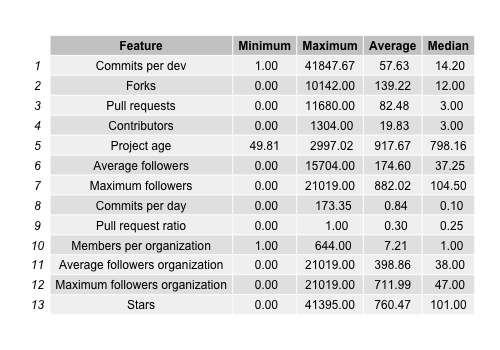
\includegraphics[width=250pt]{figures/data_summary_table}
	        \caption{The minimum value, maximum value, mean and median of all the right skewed variables}
	        \label{fig:right-skewed-features}
	    \end{figure}
        
    	\begin{LaTeXdescription}
    	\item[Countries]
    	Figure \ref{fig:country-plot} shows the countries in which the project was created.
    	As can be easily retrieved from the figure, most of the projects tend to be created in the US.
    	However, we also find a large spike for the `unknown' value, which indicate that a lot of the developers on GitHub have not specified their country of origin.
    	\item[Programming languages]
    	Figure \ref{fig:language-frequency-plot} shows the programming languages used in each of the projects in the dataset.
    	Just as with the countries, we see a big spike for the `unknown' value.
    	The reason behind this is that there are a lot of projects on GitHub that are created, but do not have any commits.
    	It is then not possible for GitHub to define a language for the project, thus we get an entry with `unknown'.
    	\item[Forks]
    	A project can be either created by a GitHub user, or be forked from an existing project.
    	Because forks tend to behave differently, for example they keep the amount of forks the original project has on GitHub, but do not get the same amount of stars, a histogram was made to see how many of the projects in the dataset are a fork.
    	This histogram can be found in Figure \ref{fig:is-fork-plot} and shows that most of the projects are not a fork.
    	\item[Project age]
    	The age of the projects can be found in Figure \ref{fig:age-plot}.
    	The age is defined as the amount of days from initial created, until January 6, 2016.
    	As can be seen from the figure, there are more projects recently created.
    	This is also in line with what you would expect, as GitHub tends to grow each year \cite{github-2013}.
    	\item[Ratio of accepted pull requests]
    	Figure \ref{fig:ratio-pull-requests-plot} shows the percentage of pull requests that was accepted per project.
    	There are two things in this plot that might attract your attention: most of the projects have a percentage of 0 accepted pull request, and there is an increase at 1 (or 100\%). 
    	Both can be easily explained: a lot of projects have a small amount of pull requests of which none are accepted, which explaints the spike around 0.
    	On the other hand, a lot of project also have one or two pull requests and have accepted these, which means that they accepted all of them.
    	Since the majority of the projects fall in these two categories, there is also an increase around 100\%.
    	\item[Number of commits per contributor]
    	Although Figure \ref{fig:nr-commit-contributor-plot} looks like a normal right skewed histogram, there is some information missing in this figure.
    	When creating the data for this plot, it was necessary to divide the amount of commits by the amount of contributors.
    	However, there can be so called `read-only mirrors' on GitHub that have commits without any contributors (for example https://github.com/cran/jomo).
    	When dividing the amount of commits by the amount of developers, this result in a division by 0 which was represented as infinity.
    	These values were not added in the plot. 
    	\end{LaTeXdescription}
        
        \todo{INSTEAD of all the pictures, add a table for all numerical values with min, max, mean, median, standard deviation}
	    %\begin{figure}[t!]
	    %    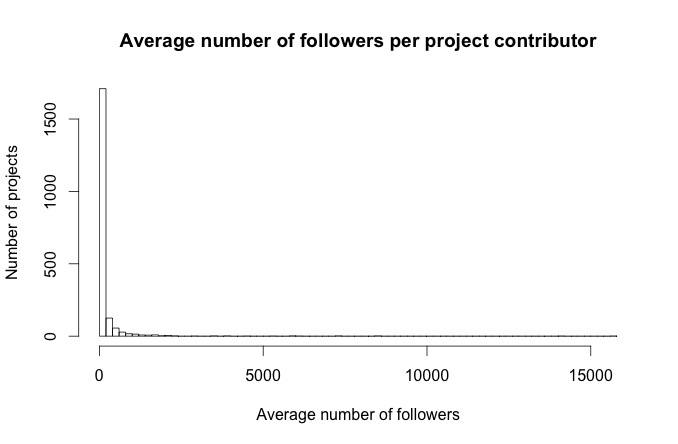
\includegraphics[width=250pt]{figures/average-number-of-followers-per-project-contributor}
	    %    \caption{The average number of followers per project contributor}
	    %    \label{fig:avg-follower-contributor-plot}
	    %\end{figure}

%	    \begin{figure}[t!]
	  %      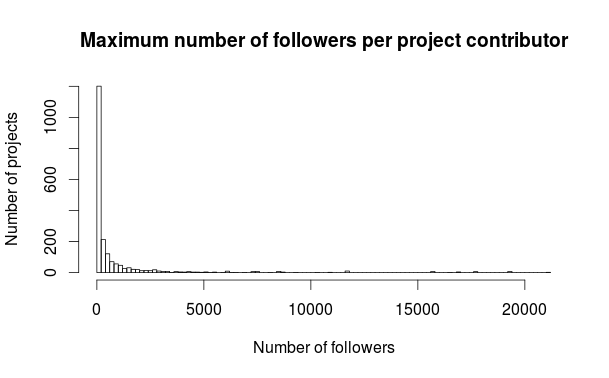
\includegraphics[width=250pt]{figures/maximum-number-of-followers-per-project-contributor}
	  %      \caption{The maximum number of followers per project contributor}
	  %      \label{fig:max-follower-contributor-plot}
	  %  \end{figure}

	   % \begin{figure}[t!]
	   %     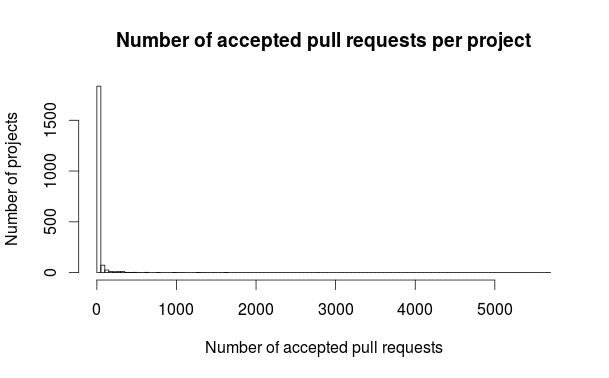
\includegraphics[width=250pt]{figures/nr-of-accepted-pull-requests-per-project}
	   %     \caption{The number of accepted pull requests per project}
	   %     \label{fig:accepted-pull-plot}
	   % \end{figure}

	   % \begin{figure}[t!]
	   %     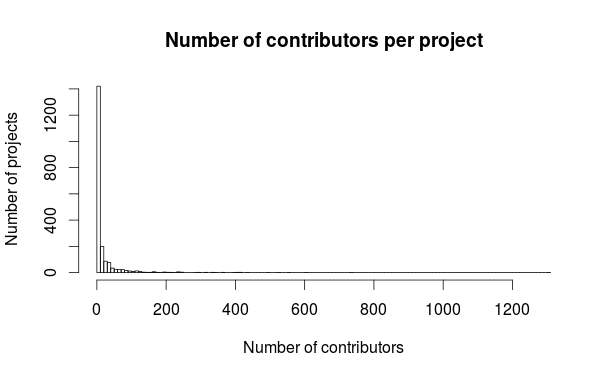
\includegraphics[width=250pt]{figures/nr-of-contributors-per-project}
	   %     \caption{The number of contributors per project}
	   %     \label{fig:nr-contributors-plot}
	   % \end{figure}

	   % \begin{figure}[t!]
	   %     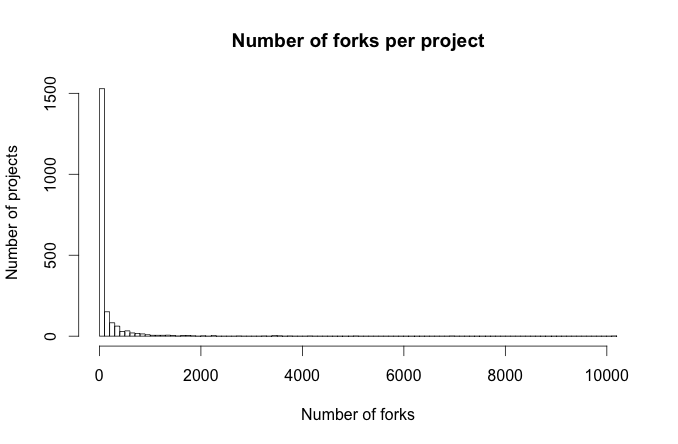
\includegraphics[width=250pt]{figures/number-of-forks-per-project}
	   %     \caption{The number of forks per project}
	   %     \label{fig:nr-forks-plot}
	   % \end{figure}

	   % \begin{figure}[t!]
	   %     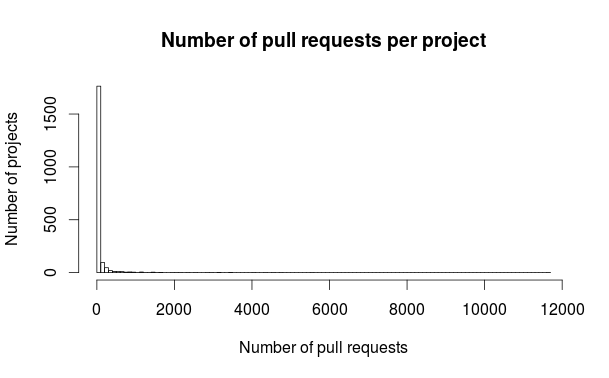
\includegraphics[width=250pt]{figures/number-of-pull-requests-per-project}
	   %     \caption{The number of pull requests per project}
	   %     \label{fig:nr-pull-requests-plot}
	   % \end{figure}

	   % \begin{figure}[t!]
	   %     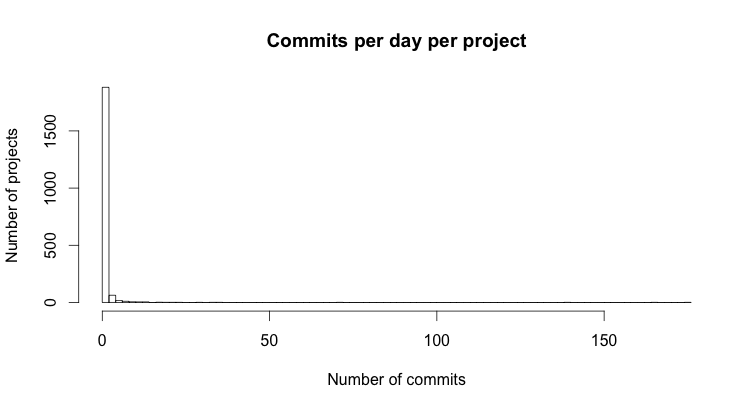
\includegraphics[width=250pt]{figures/commits-per-day-per-project}
	   %     \caption{The number of commits per day per project}
	   %     \label{fig:nr-commits-day-plot}
	   % \end{figure}

	    \begin{figure}[h!]
	        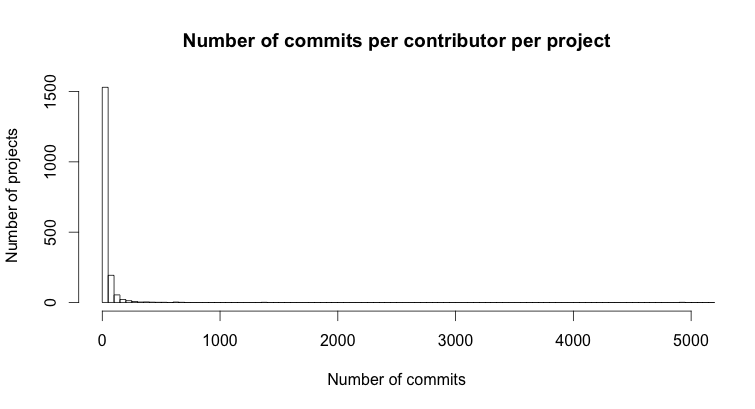
\includegraphics[width=250pt]{figures/nr-commits-per-contributor}
	        \caption{The number of commits per contributor per project}
	        \label{fig:nr-commit-contributor-plot}
	    \end{figure}

	    \begin{figure}[h!]
	        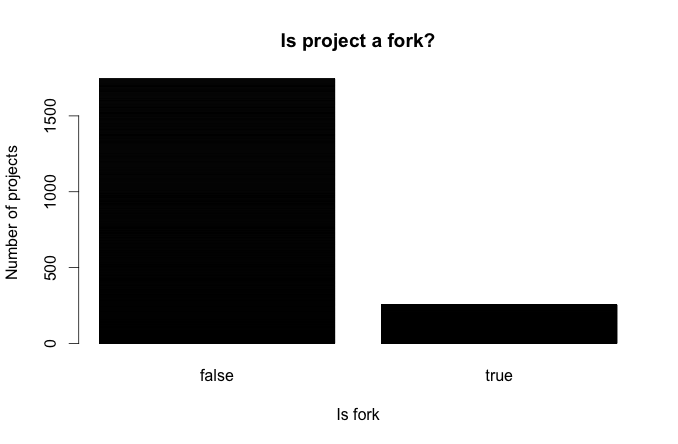
\includegraphics[width=250pt]{figures/isfork-per-project}
	        \caption{A histogram showing whether a project is a fork or not}
	        \label{fig:is-fork-plot}
	    \end{figure}

	    \begin{figure}[h!]
	        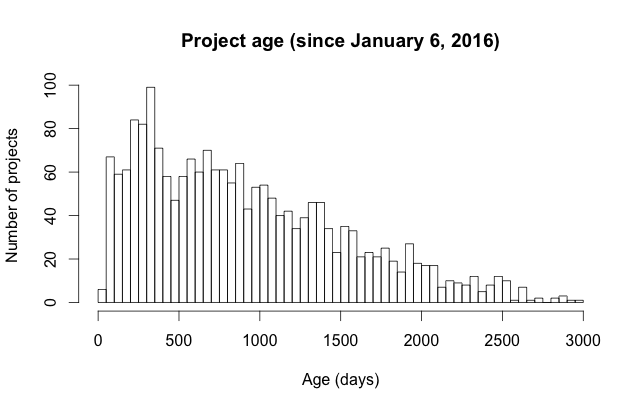
\includegraphics[width=250pt]{figures/project-age}
	        \caption{The age of the project in days from January 6, 2016}
	        \label{fig:age-plot}
	    \end{figure}

	    \begin{figure}[h]
	        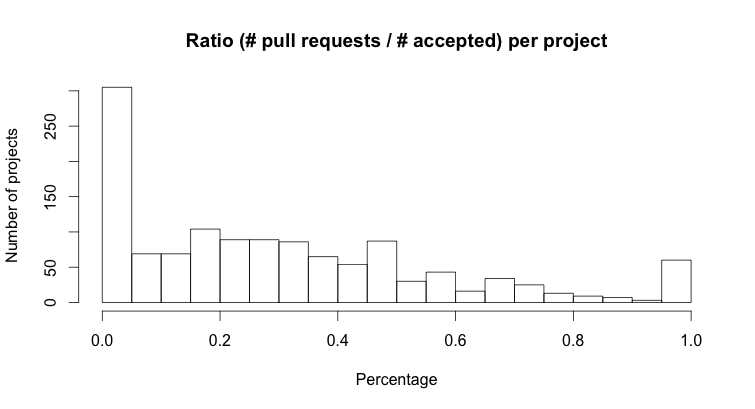
\includegraphics[width=250pt]{figures/ratio-pull-request-per-project}
	        \caption{The ratio of accepted pull requests per project}
	        \label{fig:ratio-pull-requests-plot}
	    \end{figure}

	    \begin{figure*}[t!]
	        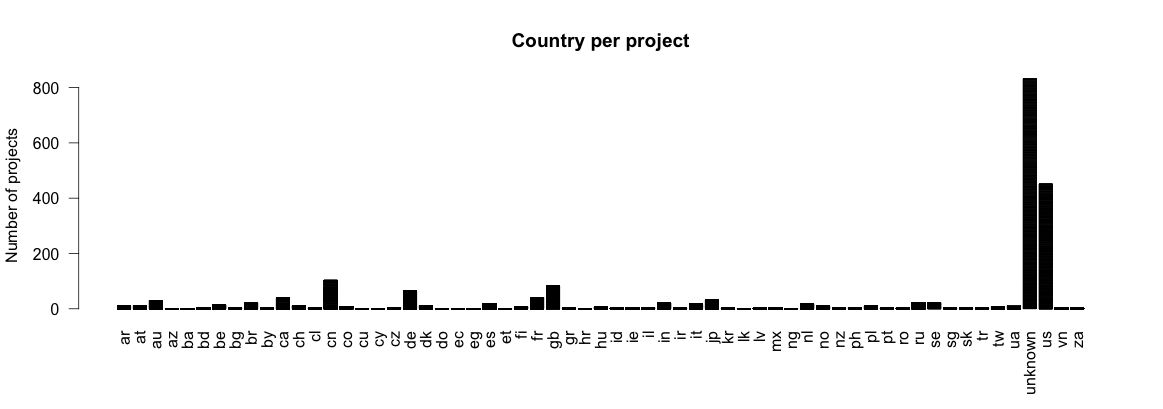
\includegraphics[width=500pt]{figures/country-per-project}
	        \caption{An overview of the countries where the project was created}
	        \label{fig:country-plot}
	    \end{figure*}

	    \begin{figure*}[t!]
	        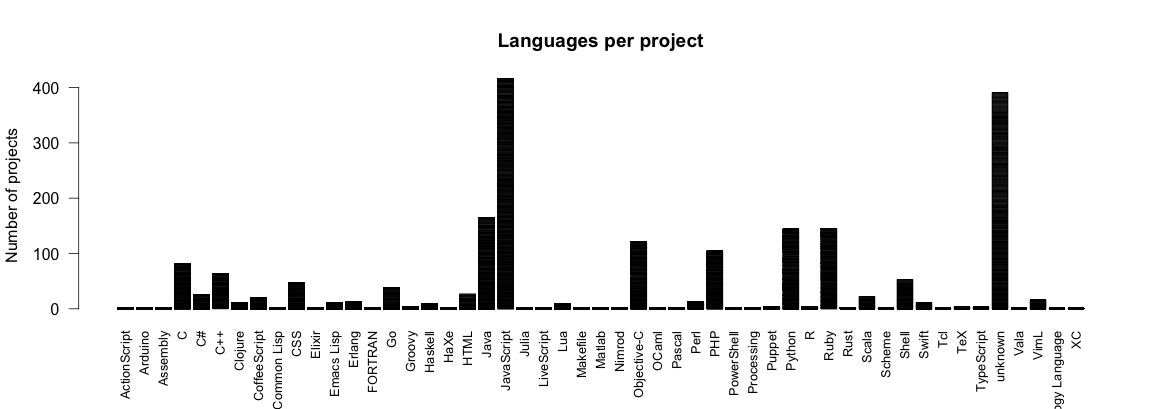
\includegraphics[width=500pt]{figures/languages-per-project}
	        \caption{An overview of the languages user per project}
	        \label{fig:language-frequency-plot}
	    \end{figure*}
    
    \subsection{Testing the model}
        \todo{Will be added later on}
